
% This LaTeX was auto-generated from MATLAB code.
% To make changes, update the MATLAB code and republish this document.

\documentclass{article}
\usepackage{graphicx}
\usepackage{color}

\sloppy
\definecolor{lightgray}{gray}{0.5}
\setlength{\parindent}{0pt}

\begin{document}

    
    
\subsection*{Contents}

\begin{itemize}
\setlength{\itemsep}{-1ex}
   \item part 1 - see jpeg image quality compression
   \item part 2 - do our own jpeg
   \item Part 3 Evaluating Quantization Tables
\end{itemize}
\begin{verbatim}
% Assignment 2
% Jan 26, 2017
% Brian Hosler & Sarah Peachey
\end{verbatim}


\subsection*{part 1 - see jpeg image quality compression}

\begin{verbatim}
pep=imread('peppers.tif');
bab=imread('baboon.tif');

imwrite(pep, 'pep90.jpg','Quality',90)
imwrite(pep, 'pep70.jpg','Quality',70)
imwrite(pep, 'pep50.jpg','Quality',50)
imwrite(pep, 'pep30.jpg','Quality',30)
imwrite(pep, 'pep10.jpg','Quality',10)

imwrite(bab, 'bab90.jpg','Quality',90)
imwrite(bab, 'bab70.jpg','Quality',70)
imwrite(bab, 'bab50.jpg','Quality',50)
imwrite(bab, 'bab30.jpg','Quality',30)
imwrite(bab, 'bab10.jpg','Quality',10)

pep_psnr=zeros(1,6);
pep_size=zeros(1,6);

temp=imfinfo('peppers.tif');
pep_size(1)=temp.FileSize;
pep_psnr(1)= psnr(pep, pep);

temp=imfinfo('pep90.jpg');
pep_size(2)=temp.FileSize;
pep_psnr(2)= psnr(imread('pep90.jpg'), pep);

temp=imfinfo('pep70.jpg');
pep_size(3)=temp.FileSize;
pep_psnr(3)= psnr(imread('pep70.jpg'), pep);

temp=imfinfo('pep50.jpg');
pep_size(4)=temp.FileSize;
pep_psnr(4)= psnr(imread('pep50.jpg'), pep);

temp=imfinfo('pep30.jpg');
pep_size(5)=temp.FileSize;
pep_psnr(5)= psnr(imread('pep30.jpg'), pep);

temp=imfinfo('pep10.jpg');
pep_size(6)=temp.FileSize;
pep_psnr(6)= psnr(imread('pep10.jpg'), pep);

figure
subplot(2,1,1)
plot(100*[1 .9 .7 .5 .3 .1],pep_size,'--o')
hold on
title('peppers - file size vs quality')
subplot(2,1,2)
plot(100*[1 .9 .7 .5 .3 .1],pep_psnr,'--o')
hold on
title('peppers - psnr vs quality')

bab_psnr=zeros(1,6);
bab_size=zeros(1,6);

temp=imfinfo('baboon.tif');
bab_size(1)=temp.FileSize;
bab_psnr(1)= psnr(bab, bab);

temp=imfinfo('bab90.jpg');
bab_size(2)=temp.FileSize;
bab_psnr(2)= psnr(imread('bab90.jpg'), bab);

temp=imfinfo('bab70.jpg');
bab_size(3)=temp.FileSize;
bab_psnr(3)= psnr(imread('bab70.jpg'), bab);

temp=imfinfo('bab50.jpg');
bab_size(4)=temp.FileSize;
bab_psnr(4)= psnr(imread('bab50.jpg'), bab);

temp=imfinfo('bab30.jpg');
bab_size(5)=temp.FileSize;
bab_psnr(5)= psnr(imread('bab30.jpg'), bab);

temp=imfinfo('bab10.jpg');
bab_size(6)=temp.FileSize;
bab_psnr(6)= psnr(imread('bab10.jpg'), bab);

figure
subplot(2,1,1)
plot(100*[1 .9 .7 .5 .3 .1],bab_size,'--o')
hold on
title('baboon - file size vs quality')
subplot(2,1,2)
plot(100*[1 .9 .7 .5 .3 .1],bab_psnr,'--o')
hold on
title('baboon - psnr vs quality')
\end{verbatim}

\includegraphics [width=4in]{lab2_01.eps}

\includegraphics [width=4in]{lab2_02.eps}


\subsection*{part 2 - do our own jpeg}

\begin{verbatim}
type('myJpgEncode.m')
type('myJpgDecode.m')
\end{verbatim}

        \color{lightgray} \begin{verbatim}
function [result] = myJpgEncode( pep,Q )
%myJpgEncode implement my own jpeg algorithm
%   using the notes 
A=zeros(size(pep)); 
stor=[];
for i=1:512/8
    for j=1:512/8
        tempA=dct2(pep(8*(i-1)+1:i*8,8*(j-1)+1:j*8)); 
        pep_quan=round(tempA./Q).*Q; 
        stor=[stor;ZigzagMtx2Vector(pep_quan)];
    end 
end

result=JPEG_entropy_encode(512,512,8,Q,stor,...
    '/Users/brianhosler/Documents/Drexel/17-18/Winter/ECES435/Winter2018/ECES435/Assignment2/Assignment2Files/',1);


end


function [pep] = myJpgDecode()
%myJpgEncode implement my own jpeg algorithm
%   using the notes 
[rowN,colN,dct_block_size,iQ,iZZDCTQIm]=JPEG_entropy_decode(...
    '/Users/brianhosler/Documents/Drexel/17-18/Winter/ECES435/Winter2018/ECES435/Assignment2/Assignment2Files/');
pep=zeros(512);
ndx=1;
for i=1:512/8
    for j=1:512/8
        pep(8*(i-1)+1:i*8,8*(j-1)+1:j*8)=idct2(Vector2ZigzagMtx(iZZDCTQIm(ndx,:)));
        ndx=ndx+1;
    end 
end 
end

\end{verbatim} \color{black}
    

\subsection*{Part 3 Evaluating Quantization Tables}

\begin{par}
luminance quantization table
\end{par} \vspace{1em}
\begin{verbatim}
Q=[16 11 10 16 24 40 51 61;...
   12 12 14 19 26 58 60 55;...
   14 13 16 24 40 57 69 56;...
   14 17 22 29 51 87 80 62;...
   18 22 37 56 68 109 103 77;...
   24 35 55 64 81 104 113 92;...
   49 64 78 87 103 121 120 101;...
   72 92 95 98 112 100 103 99];

tempQ=zeros(8);
for i=1:512/8
    for j=1:512/8
        tempQ=tempQ+abs(dct2(pep(8*(i-1)+1:i*8,8*(j-1)+1:j*8)));
    end
end
DCTs=tempQ/4096;
nrm1=max(max(DCTs))./DCTs;
Q2=double(uint8(nrm1.^.65));

stor=[];
for i=1:512/8
    for j=1:512/8
        tempA=dct2(pep(8*(i-1)+1:i*8,8*(j-1)+1:j*8));
        stor=[stor;ZigzagMtx2Vector(tempA)];
    end
end
vrnce=Vector2ZigzagMtx(var(stor));
nrm2=max(max(vrnce))./vrnce;
Q3=double(uint8(log(nrm2).^2))+1;

A=myJpgEncode( pep,Q );
jpg1=uint8(myJpgDecode());
psnr(pep,jpg1)

B=myJpgEncode( pep,Q2 );
jpg2=uint8(myJpgDecode());
psnr(pep,jpg2)

C=myJpgEncode( pep,Q3 );
jpg3=uint8(myJpgDecode());
psnr(pep,jpg3)

figure
imshow([pep,jpg1;jpg2,jpg3])
\end{verbatim}

        \color{lightgray} \begin{verbatim}/usr/local/bin/wine JPEG_entropy_encode.exe: Signal 120

ans =

   36.2761

/usr/local/bin/wine JPEG_entropy_encode.exe: Signal 120

ans =

   36.3328

/usr/local/bin/wine JPEG_entropy_encode.exe: Signal 120

ans =

   34.3979

Warning: Image is too big to fit on screen; displaying at 50% 
\end{verbatim} \color{black}
    
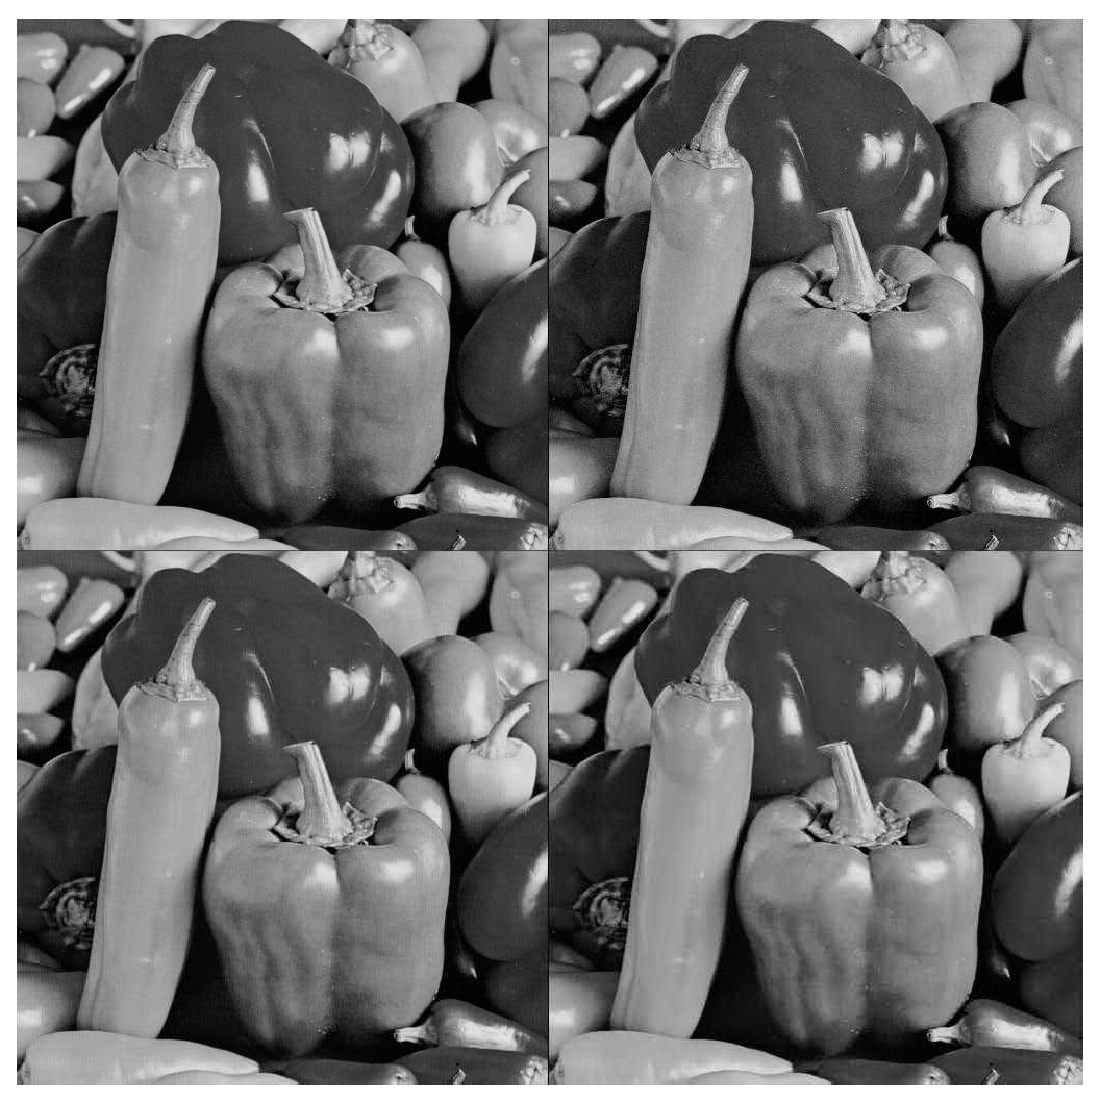
\includegraphics [width=4in]{lab2_03.eps}



\end{document}
    
